\documentclass[11pt,a4paper]{article}

%%%%%%%%%%%%%%%%%%%%%%%%%%%%%%%%%%%%%%%%%%%%%%%%%%%%%%%%%%%%%%%%%%%%%%%%
%%  Efficient Deep Learning Systems -- Lecture 3: Data-Parallel       %%
%%  Deep Learning                                                     %%
%%  Lecture notes, cleaned and typeset (design matches Lecture 1).    %%
%%  Links from the lecture slides added as footnotes / \href.         %%
%%%%%%%%%%%%%%%%%%%%%%%%%%%%%%%%%%%%%%%%%%%%%%%%%%%%%%%%%%%%%%%%%%%%%%%%

% ---- Packages ----
\usepackage[utf8]{inputenc}
\usepackage[T1]{fontenc}
\usepackage[english]{babel}

\usepackage[margin=1.1in]{geometry}
\usepackage{amsmath, amssymb, amsthm, mathtools}
\usepackage{booktabs, array}
\usepackage{enumitem}
\usepackage{xcolor}
\usepackage{graphicx}
\usepackage{epigraph}
\usepackage{csquotes}
\usepackage{tikz}
\usetikzlibrary{arrows.meta, positioning, shapes.geometric, shapes.misc,
                fit, calc, backgrounds, decorations.pathreplacing,
                patterns, matrix}
\usepackage{pgfplots}
\pgfplotsset{compat=1.18}

\usepackage[colorlinks=true, linkcolor=black!70!blue,
            citecolor=black!70!blue, urlcolor=black!40!blue]{hyperref}

% ---- Theorem environments ----
\theoremstyle{definition}
\newtheorem{definition}{Definition}[section]
\newtheorem{example}[definition]{Example}

\theoremstyle{remark}
\newtheorem*{remark}{Remark}
\newtheorem*{aside}{Aside}

\theoremstyle{plain}
\newtheorem{proposition}[definition]{Proposition}

% ---- Epigraph style ----
\setlength{\epigraphwidth}{0.6\textwidth}
\renewcommand{\epigraphflush}{flushright}
\renewcommand{\textflush}{flushright}
\renewcommand{\epigraphsize}{\small\itshape}

% ---- Small conveniences ----
\newcommand{\todo}[1]{\textcolor{red!70!black}{\textbf{[TODO: #1]}}}
\DeclareMathOperator*{\argmin}{arg\,min}
\newcommand{\GPU}[1]{\mathrm{GPU}_{#1}}
\newcommand{\grad}{\nabla_{\theta}}
\newcommand{\Loss}{\mathcal{L}}
\newcommand{\bigO}{\mathcal{O}}
\newcommand{\allreduce}{\textsc{AllReduce}}
\newcommand{\reduce}{\textsc{Reduce}}

% ---- Title ----
\title{\textbf{Efficient Deep Learning Systems} \\[0.3em]
       \large Lecture 3 --- Data-Parallel Deep Learning: \\
       Collective Communication, Decentralization, and Compression}
\author{Lecture notes}
\date{}

\begin{document}
\sloppy
\maketitle

\begin{abstract}
\noindent
These notes develop the theory and practice of \emph{data-parallel} deep
learning---the coordination of many heterogeneous accelerators (CPUs,
GPUs, TPUs, NPUs) around a single optimization problem. We begin with an
abstract model of processes communicating via channels, proceed to the
na\"ive host--device training loop, and progressively refine the picture
through centralized reductions, tree- and ring-based \allreduce, torus
topologies, and decentralized gossip protocols. The exposition culminates
in modern practical techniques: PyTorch \texttt{DistributedDataParallel},
error-feedback compression, and PowerSGD. The guiding theme is a
recurring tension: raw arithmetic capacity grows readily, but
\emph{communication}---the silent partner of every distributed
algorithm---does not, and its costs ultimately dictate the shape of every
scalable system.
\end{abstract}

\tableofcontents
\bigskip
\hrule
\bigskip

%%%%%%%%%%%%%%%%%%%%%%%%%%%%%%%%%%%%%%%%%%%%%%%%%%%%%%%%%%%%%%%%%%%%%%%%
\section{Motivation: The Arithmetic of Scale}
%%%%%%%%%%%%%%%%%%%%%%%%%%%%%%%%%%%%%%%%%%%%%%%%%%%%%%%%%%%%%%%%%%%%%%%%

Modern deep learning is, in a precise sense, a problem of
\emph{orchestration}. A single large language model may have hundreds of
billions of parameters; training it to convergence requires a number of
floating-point operations that no single processor can reasonably supply
in a human lifetime. The object of these lectures is therefore to
understand how one may coordinate a large, possibly heterogeneous
population of processing units---CPUs, GPUs, TPUs, NPUs, and various
special-purpose accelerators, some of which lack a dedicated
floating-point unit---so that they operate as a single computational
organism.

\subsection{Why Parallelize?}

The parallelization of learning algorithms is not peculiar to neural
networks: the same principles apply to gradient boosting
(\textsc{XGBoost} is a familiar example) and, more generally, to any
optimization procedure with enough mathematical structure to be
decomposed across workers. When we partition a computation across several
nodes, one of two philosophical stances is available.

\begin{enumerate}[label=(\roman*), leftmargin=2em, itemsep=2pt]
  \item \textbf{Strict preservation of semantics.} The distributed
        algorithm is bitwise (or at least mathematically) equivalent to
        its serial counterpart. Every theoretical guarantee of the
        single-machine algorithm transfers intact.
  \item \textbf{Controlled relaxation.} Certain invariants---strict
        associativity of floating-point summation, synchrony, or the
        identity of gradients used---are deliberately relaxed, in
        exchange for throughput gains that outweigh the incurred
        statistical cost.
\end{enumerate}

In practice the second stance dominates. An asynchronous scheme that
trains twice as fast while sacrificing a few percent of convergence rate
is often the correct engineering choice. The art lies in \emph{knowing
what one is trading away}.

\subsection{The Thread-Count Curve}

A simple empirical picture frames the discussion. Consider the training
time of \textsc{XGBoost} as a function of the number of available worker
threads, measured on two hardware configurations (a dual Xeon E5-2695v2
server and an NVIDIA Titan X).

\begin{center}
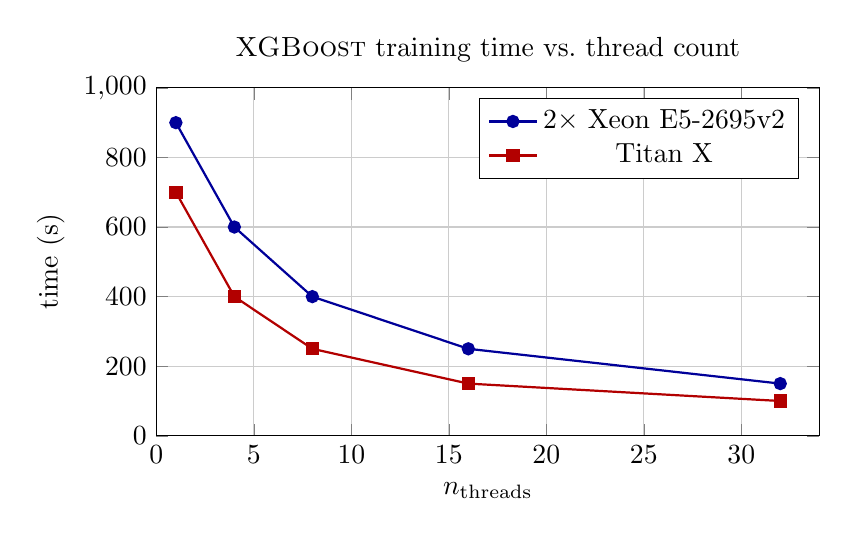
\begin{tikzpicture}
\begin{axis}[
    width=10cm, height=6cm,
    title={\textsc{XGBoost} training time vs.\ thread count},
    xlabel={$n_{\text{threads}}$},
    ylabel={time (s)},
    xmin=0, xmax=34, ymin=0, ymax=1000,
    legend pos=north east,
    grid=both,
    major grid style={black!20},
    minor grid style={black!8}
]
\addplot[color=blue!60!black, mark=*, thick] coordinates
    {(1,900) (4,600) (8,400) (16,250) (32,150)};
\addplot[color=red!70!black, mark=square*, thick] coordinates
    {(1,700) (4,400) (8,250) (16,150) (32,100)};
\legend{2$\times$ Xeon E5-2695v2, Titan X}
\end{axis}
\end{tikzpicture}
\par\smallskip
{\small Schematic redraw of the slide's plot; the plotted values are
illustrative, not the original measurements.}
\end{center}

Two observations deserve emphasis. First, increasing parallelism reliably
decreases wall-clock time. Second, the returns diminish: each doubling of
threads buys a smaller fraction of the remaining time, and the curve
asymptotes. This gap between ideal linear speed-up and realized speed-up
is the central object of study throughout these notes.

\subsection{The Scaling of Language Models}

Between 2018 and 2022 the parameter count of flagship language models grew
by roughly four orders of magnitude---from \textsc{Bert} (hundreds of
millions) to \textsc{Gpt-3} and its successors (hundreds of billions),
culminating today in the trillion-parameter regime. Empirical scaling laws
support the observation that model quality improves predictably with joint
increases in parameter count, dataset size, and compute budget.

\begin{center}
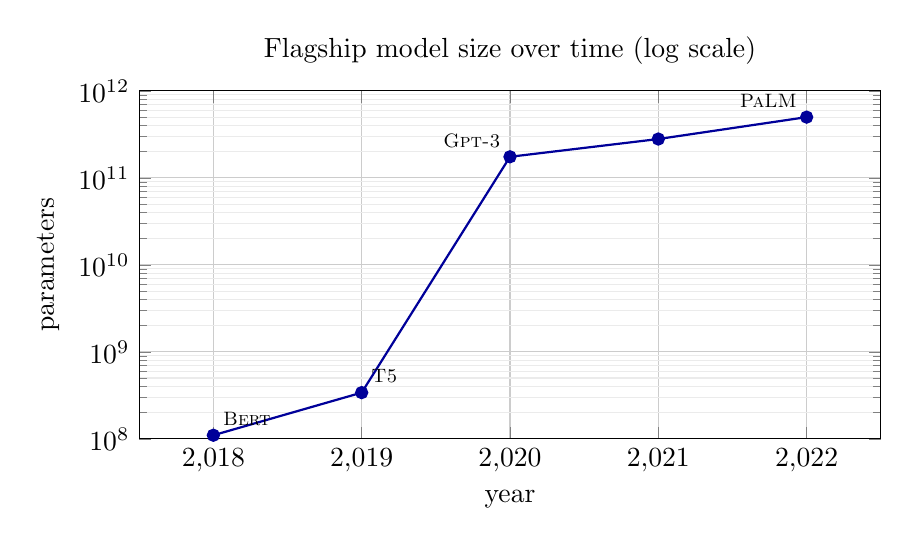
\begin{tikzpicture}
\begin{axis}[
    width=11cm, height=6cm,
    title={Flagship model size over time (log scale)},
    xlabel={year},
    ylabel={parameters},
    xmin=2017.5, xmax=2022.5,
    ymin=1e8, ymax=1e12,
    ymode=log,
    xtick={2018,2019,2020,2021,2022},
    grid=both,
    major grid style={black!20},
    minor grid style={black!8}
]
\addplot[color=blue!60!black, mark=*, thick] coordinates
    {(2018, 1.1e8) (2019, 3.4e8) (2020, 1.75e11) (2021, 2.8e11) (2022, 5.0e11)};
\node[anchor=south west] at (axis cs: 2018, 1.1e8) {\scriptsize \textsc{Bert}};
\node[anchor=south west] at (axis cs: 2019, 3.4e8) {\scriptsize \textsc{T5}};
\node[anchor=south east] at (axis cs: 2020, 1.75e11) {\scriptsize \textsc{Gpt-3}};
\node[anchor=south east] at (axis cs: 2022, 5.0e11) {\scriptsize \textsc{PaLM}};
\end{axis}
\end{tikzpicture}
\par\smallskip
{\small Schematic redraw of the slide's trend plot; values are approximate.}
\end{center}

\subsection{Hardware, Open Models, and the Need to Train}

The dominant training records---\textsc{Bert-Large} in $47$ minutes on a
$1024$-GPU DGX SuperPOD, $67$ minutes on $512$ GPUs, and $236$ minutes on
$256$ GPUs---make plain that state-of-the-art pretraining is the province
of hyperscalers. Yet even with extraordinary open-source checkpoints
freely available, most organizations still need to train. Two reasons
recur:

\begin{description}[leftmargin=1.5em, style=nextline]
  \item[Domain adaptation.] General-purpose models lack the nuance of
        proprietary corpora, specialized vocabularies, or minority
        languages.
  \item[Fine-tuning.] Even when full pretraining is forgone, adapting a
        pretrained model to a specific task or language remains
        indispensable.
\end{description}

The practical question then sharpens: \emph{how do we train effectively on
a handful of servers when the original creators used thousands?}
Answering that question is the business of the remainder of these notes.

%%%%%%%%%%%%%%%%%%%%%%%%%%%%%%%%%%%%%%%%%%%%%%%%%%%%%%%%%%%%%%%%%%%%%%%%
\section{An Abstract Model: Processes and Channels}
%%%%%%%%%%%%%%%%%%%%%%%%%%%%%%%%%%%%%%%%%%%%%%%%%%%%%%%%%%%%%%%%%%%%%%%%

Before engaging with GPUs directly, we require a language-agnostic
abstraction that describes how concurrent workers cooperate. The right
vocabulary is process-oriented: its primitives are \emph{processes} that
compute, and \emph{channels} through which they exchange data.

\subsection{Threads, Processes, and Context}

Parallelism at the operating-system level is obtained through two
principal mechanisms: \emph{threads} and \emph{processes}. High-level
languages (\textsc{C++}, \textsc{Python}) expose both, and each has a
legitimate role. Central to the distinction is the notion of
\emph{context}: the state that defines a unit of execution---its
registers, stack pointer, and program counter. Threads share an address
space and thus exchange context cheaply; processes do not, and pay a
heavier context-switching cost in return for stronger isolation.

Lightweight alternatives---greenlets, coroutines, goroutines---offer
cooperative scheduling within a single OS-level process, and each has its
own trade-offs. For our purposes a \emph{process-and-channel} abstraction
suffices and, crucially, translates well across languages and across the
boundary from a single server to a cluster.

\subsection{The Process Abstraction}

\begin{definition}[Process]
A \emph{process} is a program in execution. It is characterized by three
properties: it runs code; it is allocated a private memory region; and
\emph{no other process may access that memory directly}.
\end{definition}

Consider a linear sequence of process-invocations
$\mathsf{foo} \to \mathsf{bar} \to \mathsf{baz} \to \mathsf{qux}$, with
time flowing left to right:

\begin{center}
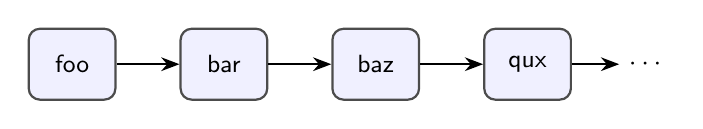
\begin{tikzpicture}[
    box/.style={rectangle, rounded corners, draw=black!70, thick,
                fill=blue!6, minimum width=1.1cm, minimum height=.9cm,
                font=\small\sffamily},
    arr/.style={-Stealth, thick},
    node distance=8mm
]
  \node[box] (foo) {foo};
  \node[box, right=of foo] (bar) {bar};
  \node[box, right=of bar] (baz) {baz};
  \node[box, right=of baz] (qux) {qux};
  \node[right=6mm of qux] (dots) {$\cdots$};
  \draw[arr] (foo) -- (bar);
  \draw[arr] (bar) -- (baz);
  \draw[arr] (baz) -- (qux);
  \draw[arr] (qux) -- (dots);
\end{tikzpicture}
\end{center}

The question immediately arises: given isolation, how do such processes
cooperate? Setting aside exotic mechanisms (shared memory, kernel
backdoors), the canonical answer is the \emph{channel}.

\subsection{Channels (Pipes)}

\begin{definition}[Channel]
A \emph{channel} (or \emph{pipe}) is a high-level abstraction for
inter-process data exchange. It may be realized by a UNIX pipe, a TCP
connection, a specialized ring buffer, or any equivalent transport.
\end{definition}

The behaviour of a channel is specified along two axes:
\emph{reliability} (is delivery guaranteed?) and \emph{synchronization}
(must the sender wait for the receiver?). The default model we adopt
throughout is \emph{reliable and asynchronous}.

\begin{proposition}[Complexity of message exchange]
Both the time and space cost of sending a message of length $L$ over a
channel are $\bigO(L)$.
\end{proposition}

\begin{remark}[Asynchronous read and write]
In the asynchronous model, a producer may write to a channel and
immediately resume its own work without waiting for the consumer. A
consumer that reads from an empty channel blocks until data arrives; this
blocking is the synchronization mechanism that keeps producer and consumer
logically coupled despite proceeding at independent speeds. An accurate
mental image is not the telephone call (synchronous) but the SMS message
(asynchronous): the sender is not inconvenienced by the recipient's
momentary unavailability.
\end{remark}

A simple topology illustrates the idea. Process~$A$ runs an internal
pipeline $\mathsf{foo} \to \mathsf{bar} \to \mathsf{baz} \to \mathsf{qux}$
that ultimately produces \textsf{result}; Process~$B$, running in
parallel, consumes intermediate values via channels to drive its own
pipeline $\mathsf{func} \to \mathsf{otherfunc}$.

\begin{center}
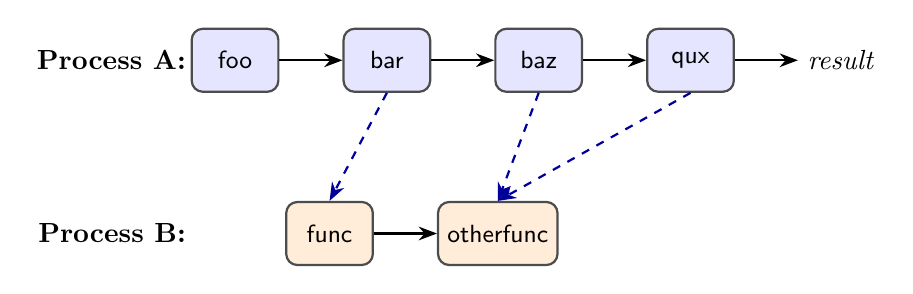
\begin{tikzpicture}[
    node distance=6mm and 8mm,
    box/.style={rectangle, rounded corners, draw=black!70, thick,
                minimum width=1.1cm, minimum height=.8cm,
                font=\small\sffamily},
    arr/.style={-Stealth, thick}]
  % Process A
  \node[anchor=east] at (-.5,0) {\textbf{Process A:}};
  \node[box, fill=blue!10] (foo)  at (0,0)   {foo};
  \node[box, fill=blue!10, right=of foo] (bar) {bar};
  \node[box, fill=blue!10, right=of bar] (baz) {baz};
  \node[box, fill=blue!10, right=of baz] (qux) {qux};
  \node[right=of qux] (result) {\textit{result}};
  \draw[arr] (foo)--(bar); \draw[arr] (bar)--(baz);
  \draw[arr] (baz)--(qux); \draw[arr] (qux)--(result);

  % Process B
  \node[anchor=east] at (-.5,-2.2) {\textbf{Process B:}};
  \node[box, fill=orange!15] (func) at (1.2,-2.2) {func};
  \node[box, fill=orange!15, right=of func] (otherfunc) {otherfunc};
  \draw[arr] (func)--(otherfunc);

  % Cross-process channels
  \draw[arr, dashed, blue!60!black] (bar.south) -- (func.north);
  \draw[arr, dashed, blue!60!black] (baz.south) -- (otherfunc.north);
  \draw[arr, dashed, blue!60!black] (qux.south) -- (otherfunc.north);
\end{tikzpicture}
\end{center}

This picture---isolated processes communicating over asynchronous
channels---is the foundation on which every subsequent construction
rests.

%%%%%%%%%%%%%%%%%%%%%%%%%%%%%%%%%%%%%%%%%%%%%%%%%%%%%%%%%%%%%%%%%%%%%%%%
\section{The Na\"ive Data-Parallel Training Loop}
%%%%%%%%%%%%%%%%%%%%%%%%%%%%%%%%%%%%%%%%%%%%%%%%%%%%%%%%%%%%%%%%%%%%%%%%

We now specialize the process/channel picture to neural-network training.
The goal is concrete: partition the computation of a single gradient
across several accelerators, so that the wall-clock time of one training
step shrinks with the number of available devices.

\subsection{Setting and Objectives}

In data parallelism the model parameters $\theta$ are \emph{replicated}
on every device; the training data are \emph{sharded}---each device
receives a distinct slice of the batch. This is the defining contrast
with \emph{model parallelism}, in which $\theta$ itself is partitioned
across devices. Scaling by enlarging the batch is the first lever; when a
batch saturates the memory of a single GPU (a batch size of 128 is a
common ceiling), splitting the batch across multiple devices becomes the
only remaining option.

\subsection{The Host--Device Dance}

A single step of na\"ive data-parallel training proceeds in five phases.
(The slides cite the parameter-server paper of Li et al., \emph{Scaling
Distributed Machine Learning with the Parameter Server} (OSDI 2014), for
this architecture.\footnote{\url{https://www.cs.cmu.edu/~muli/file/parameter_server_osdi14.pdf}})

\begin{enumerate}[leftmargin=1.8em, itemsep=2pt, label=\textbf{\arabic*.}]
  \item \textbf{Replicate and scatter.} The host (CPU) holds the master
        parameters $\theta$ and the global batch $X$. It
        \emph{replicates} $\theta$ to every device and \emph{scatters}
        the batch as $X_1,\ldots,X_N$, one shard per GPU.
  \item \textbf{Forward pass.} Each device $i$ computes
        $\Loss(X_i;\theta)$ using its local copy of $\theta$.
  \item \textbf{Backward pass.} Each device computes the local gradient
        $\grad \Loss(X_i)$.
  \item \textbf{Reduction.} Local gradients are summed (or averaged) into
        a single global gradient
        $\grad \Loss_{\text{tot}} = \sum_{i=1}^N \grad \Loss(X_i)$.
  \item \textbf{Update.} An optimizer step produces
        $\theta_{\text{new}} = \theta - \eta \,\grad \Loss_{\text{tot}}$,
        which is then broadcast back to every device.
\end{enumerate}

The diagram below captures the flow. The host acts as both parameter
server and reduction point; each GPU executes its own forward/backward
pipeline on its shard.

\begin{center}
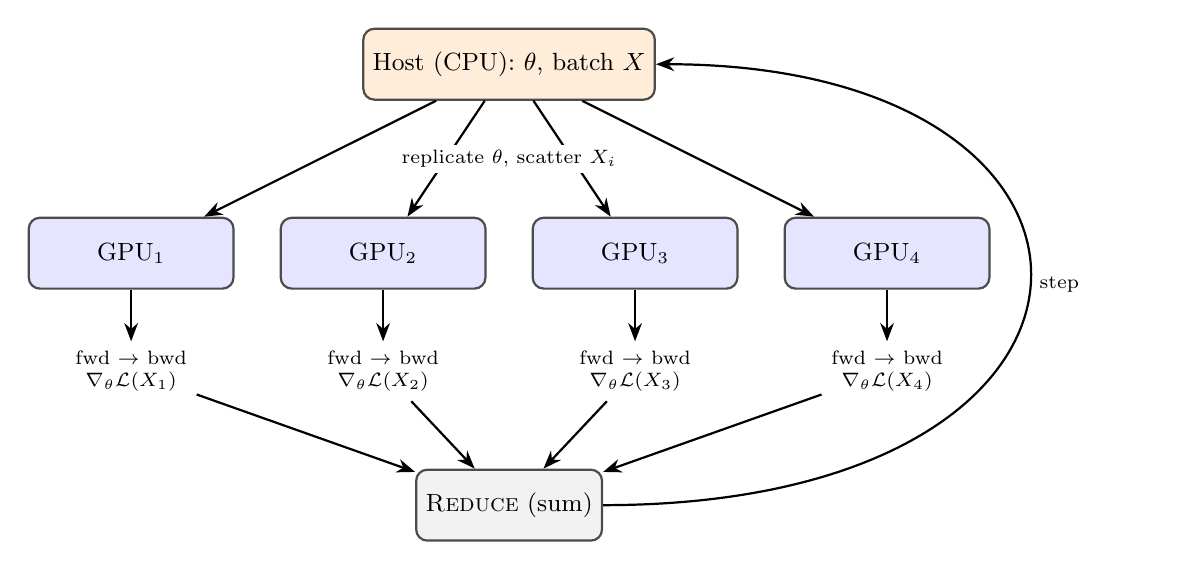
\begin{tikzpicture}[
  host/.style={rectangle, rounded corners, draw=black!70, thick,
               fill=orange!15, minimum width=3.4cm, minimum height=.9cm,
               font=\small},
  dev/.style ={rectangle, rounded corners, draw=black!70, thick,
               fill=blue!10, minimum width=2.6cm, minimum height=.9cm,
               font=\small},
  redx/.style={rectangle, rounded corners, draw=black!70, thick,
               fill=gray!10, minimum width=2cm, minimum height=.9cm,
               font=\small},
  arr/.style ={-Stealth, thick}]

  \node[host] (cpu) at (0,0) {Host (CPU): $\theta$, batch $X$};

  \node[dev] (g1) at (-4.8,-2.4) {$\GPU{1}$};
  \node[dev] (g2) at (-1.6,-2.4) {$\GPU{2}$};
  \node[dev] (g3) at ( 1.6,-2.4) {$\GPU{3}$};
  \node[dev] (g4) at ( 4.8,-2.4) {$\GPU{4}$};

  \foreach \g in {g1,g2,g3,g4} {
     \draw[arr] (cpu) -- (\g);
  }
  \node[font=\scriptsize, fill=white, inner sep=2pt] at (0,-1.2)
        {replicate $\theta$, scatter $X_i$};

  \node[font=\scriptsize, align=center] (c1) at (-4.8,-3.9) {fwd $\to$ bwd \\ $\grad\Loss(X_1)$};
  \node[font=\scriptsize, align=center] (c2) at (-1.6,-3.9) {fwd $\to$ bwd \\ $\grad\Loss(X_2)$};
  \node[font=\scriptsize, align=center] (c3) at ( 1.6,-3.9) {fwd $\to$ bwd \\ $\grad\Loss(X_3)$};
  \node[font=\scriptsize, align=center] (c4) at ( 4.8,-3.9) {fwd $\to$ bwd \\ $\grad\Loss(X_4)$};
  \draw[arr] (g1)--(c1); \draw[arr] (g2)--(c2);
  \draw[arr] (g3)--(c3); \draw[arr] (g4)--(c4);

  \node[redx] (red) at (0,-5.6) {\reduce\ (sum)};
  \draw[arr] (c1) -- (red); \draw[arr] (c2) -- (red);
  \draw[arr] (c3) -- (red); \draw[arr] (c4) -- (red);

  \draw[arr] (red.east) .. controls (8.3,-5.6) and (8.3,0) ..
       node[pos=.5, right, font=\scriptsize]{step} (cpu.east);
\end{tikzpicture}
\end{center}

\subsection{CPU--GPU Pipelining}

A correct implementation of the diagram above is not automatically an
\emph{efficient} one. The paradigmatic pathology is the idle GPU: while
the CPU prepares the next batch---decoding images, tokenizing text,
shuffling indices---the GPU waits with nothing to do. Symmetrically, the
CPU may idle while the GPU computes. The cure is to treat CPU and GPU as
two stages of a \emph{pipeline}, overlapping each stage's work with the
other's.

In PyTorch, this overlap is delivered by the \texttt{DataLoader} through
the \texttt{num\_workers} parameter. Setting \texttt{num\_workers}
$> 0$ spawns separate worker processes that prefetch and preprocess the
next batch concurrently with the current GPU computation. In ordinary
configurations one or two workers suffice to keep the GPU continuously
fed.

\begin{remark}
The location of the reduction and the optimizer step is not fixed by the
abstract model. Placing them on GPU~0 instead of the CPU is
algorithmically identical but frequently faster, because intra-GPU
bandwidth and specialized collective primitives outperform the round-trip
to host memory.
\end{remark}

\subsection{Where the Na\"ive Design Fails}

The na\"ive architecture breaks down at scale for two related reasons:

\begin{itemize}[leftmargin=1.5em, itemsep=2pt]
  \item \textbf{Gradient exchange.} Funneling every gradient through a
        single aggregator makes the aggregator's bandwidth the ceiling on
        system throughput. At thousands of devices the aggregator drowns.
  \item \textbf{Model transfer.} Broadcasting $\theta_{\text{new}}$ to
        every device after every step is prohibitively expensive when
        $\theta$ has $10^{11}$--$10^{12}$ entries.
\end{itemize}

Both failures push us toward collective-communication patterns that do not
rely on a central hub---the province of the next section.

%%%%%%%%%%%%%%%%%%%%%%%%%%%%%%%%%%%%%%%%%%%%%%%%%%%%%%%%%%%%%%%%%%%%%%%%
\section{Collective Communication: \allreduce\ in its Many Forms}
%%%%%%%%%%%%%%%%%%%%%%%%%%%%%%%%%%%%%%%%%%%%%%%%%%%%%%%%%%%%%%%%%%%%%%%%

\subsection{The \allreduce\ Primitive}

\begin{definition}[\allreduce]
Let $N$ nodes each hold a vector $v_i \in \mathbb{R}^d$. An \allreduce\ is
a collective operation whose output, delivered to \emph{every}
participant, is the reduction (typically a sum or mean) of all inputs:
\[
   \text{output at node } i \;=\; \bigoplus_{j=1}^{N} v_j,
   \qquad i = 1,\ldots,N,
\]
where $\oplus$ is an associative, commutative operator (e.g.\ $+$).
\end{definition}

\allreduce\ is the right primitive for synchronized data parallelism: if
every device begins a step with identical $\theta$ and receives identical
aggregated gradients, then every device computes identical
$\theta_{\text{new}}$, and the cluster remains in lockstep with no
central server.

\subsection{Synchronized SGD via \allreduce}

The complete workflow on each device $i$, with initial $\theta$ shared
across the cluster, is
\[
   \GPU{i} \;\xrightarrow{\theta,\,X_i}\;
   \text{forward} \;\xrightarrow{}\;
   \text{backward} \;\xrightarrow{}\;
   \grad \Loss(X_i) \;\xrightarrow{\allreduce}\;
   \overline{\grad \Loss} \;\xrightarrow{\text{step}}\;
   \theta_{\text{new}},
\]
where
$\overline{\grad \Loss} = \tfrac{1}{N}\sum_{i=1}^N \grad \Loss(X_i)$.
Because the update rule
\[
   \theta_{\text{new}} \;=\; \theta \;-\; \eta \cdot \overline{\grad \Loss}
\]
is identical on every device, and because every device began with the same
$\theta$, consistency is maintained without explicit broadcasting of
parameters. This is the all-reduce data-parallel scheme popularized by
Goyal et al., \href{https://arxiv.org/abs/1706.02677}{\textit{Accurate,
Large Minibatch SGD: Training ImageNet in 1 Hour}}.

\begin{remark}[Floating-point associativity]
In exact arithmetic the order of summation is immaterial; in
floating-point arithmetic it is not. A ``sum'' computed in different
orders on different devices produces different bits---small discrepancies
that, compounded over many iterations, can silently desynchronize a
cluster. A correct \allreduce\ implementation (ring, tree, or otherwise)
is \emph{deterministic}: every device receives bit-for-bit the same
reduced value.
\end{remark}

\subsection{Na\"ive Centralized \allreduce}

The pedagogical starting point is the centralized implementation: every
GPU ships its full local vector to a designated aggregator, which sums and
broadcasts.

\begin{center}
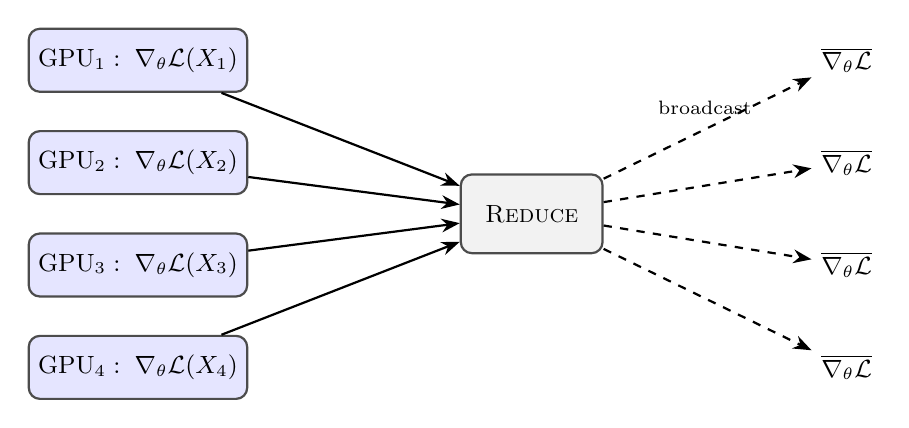
\begin{tikzpicture}[
  g/.style={rectangle, rounded corners, draw=black!70, thick,
            minimum width=2.1cm, minimum height=.8cm,
            fill=blue!10, font=\small},
  arr/.style={-Stealth, thick}]
  \node[g] (g1) at (0, 0)    {$\GPU{1}:\;\grad\Loss(X_1)$};
  \node[g] (g2) at (0,-1.3)  {$\GPU{2}:\;\grad\Loss(X_2)$};
  \node[g] (g3) at (0,-2.6)  {$\GPU{3}:\;\grad\Loss(X_3)$};
  \node[g] (g4) at (0,-3.9)  {$\GPU{4}:\;\grad\Loss(X_4)$};
  \node[rectangle, rounded corners, draw=black!70, thick, fill=gray!10,
        minimum width=1.8cm, minimum height=1cm, font=\small]
        (sum) at (5,-1.95) {\reduce};
  \draw[arr] (g1) -- (sum); \draw[arr] (g2) -- (sum);
  \draw[arr] (g3) -- (sum); \draw[arr] (g4) -- (sum);

  \node[font=\small] (b1) at (9, 0)    {$\overline{\grad\Loss}$};
  \node[font=\small] (b2) at (9,-1.3)  {$\overline{\grad\Loss}$};
  \node[font=\small] (b3) at (9,-2.6)  {$\overline{\grad\Loss}$};
  \node[font=\small] (b4) at (9,-3.9)  {$\overline{\grad\Loss}$};
  \draw[arr, dashed] (sum) -- (b1); \draw[arr, dashed] (sum) -- (b2);
  \draw[arr, dashed] (sum) -- (b3); \draw[arr, dashed] (sum) -- (b4);
  \node[font=\scriptsize] at (7.2,-0.6) {broadcast};
\end{tikzpicture}
\end{center}

The aggregator must handle $N$ incoming and $N$ outgoing streams, and the
other devices idle while it works. Both the link into the aggregator and
the aggregator itself are bottlenecks. We need patterns that \emph{share}
the communication load.

\subsection{Tree-\allreduce}

A tree reduction pairs devices recursively. In the four-device case,
GPU~1 and GPU~2 exchange and sum their vectors; GPU~3 and GPU~4 do
likewise; then the two partial sums are combined; finally the global sum
is broadcast back down the tree.

\begin{center}
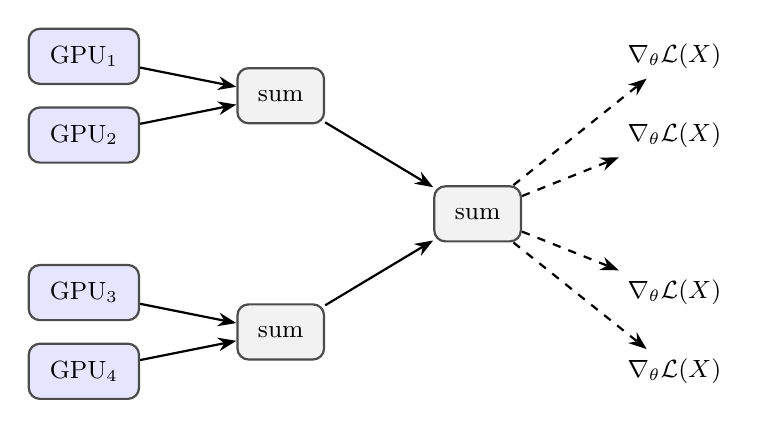
\begin{tikzpicture}[
  g/.style={rectangle, rounded corners, draw=black!70, thick,
            minimum width=1.4cm, minimum height=.7cm,
            fill=blue!10, font=\small},
  s/.style={rectangle, rounded corners, draw=black!70, thick, fill=gray!10,
            minimum width=1.1cm, minimum height=.7cm, font=\small},
  arr/.style={-Stealth, thick}]

  \node[g] (g1) at (0,2)    {$\GPU{1}$};
  \node[g] (g2) at (0,1)    {$\GPU{2}$};
  \node[g] (g3) at (0,-1)   {$\GPU{3}$};
  \node[g] (g4) at (0,-2)   {$\GPU{4}$};

  \node[s] (s12) at (2.5, 1.5)  {sum};
  \node[s] (s34) at (2.5,-1.5)  {sum};
  \node[s] (sT)  at (5, 0)      {sum};

  \draw[arr] (g1) -- (s12); \draw[arr] (g2) -- (s12);
  \draw[arr] (g3) -- (s34); \draw[arr] (g4) -- (s34);
  \draw[arr] (s12) -- (sT); \draw[arr] (s34) -- (sT);

  \node[font=\small] (b1) at (7.5, 2)  {$\grad\Loss(X)$};
  \node[font=\small] (b2) at (7.5, 1)  {$\grad\Loss(X)$};
  \node[font=\small] (b3) at (7.5,-1)  {$\grad\Loss(X)$};
  \node[font=\small] (b4) at (7.5,-2)  {$\grad\Loss(X)$};
  \draw[arr, dashed] (sT) -- (b1); \draw[arr, dashed] (sT) -- (b2);
  \draw[arr, dashed] (sT) -- (b3); \draw[arr, dashed] (sT) -- (b4);
\end{tikzpicture}
\end{center}

The tree moves the serial bottleneck from a single node to a height of
$\log_2 N$ levels, each of which can execute in parallel within itself.

\subsection{Ring-\allreduce}

The \emph{ring} is the dominant pattern in modern large-scale training.
Each of $N$ GPUs is a node on a logical ring; each node talks only to its
two neighbours. The vector is partitioned into $N$ chunks, and the
algorithm proceeds in two phases.

\begin{description}[leftmargin=1.5em, style=nextline]
  \item[Phase~I: Scatter-reduce.] In $N-1$ steps, chunk~$k$ is passed
        around the ring in such a way that after the phase, each GPU
        holds the complete sum of \emph{one} chunk.
  \item[Phase~II: All-gather.] In another $N-1$ steps, the fully reduced
        chunks are circulated so that every GPU holds the full reduced
        vector.
\end{description}

\begin{center}
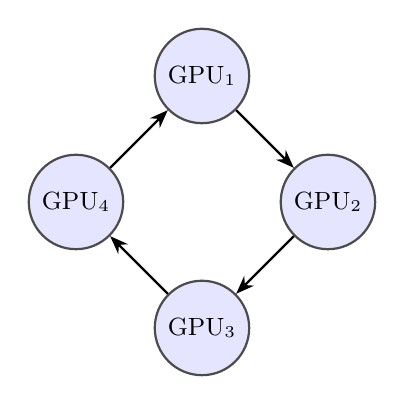
\begin{tikzpicture}[
  g/.style={circle, draw=black!70, thick, minimum size=1.1cm,
            fill=blue!10, font=\small},
  arr/.style={-Stealth, thick}]
  \node[g] (g1) at (0,1.6)   {$\GPU{1}$};
  \node[g] (g2) at (1.6,0)   {$\GPU{2}$};
  \node[g] (g3) at (0,-1.6)  {$\GPU{3}$};
  \node[g] (g4) at (-1.6,0)  {$\GPU{4}$};
  \draw[arr] (g1) -- (g2);
  \draw[arr] (g2) -- (g3);
  \draw[arr] (g3) -- (g4);
  \draw[arr] (g4) -- (g1);
\end{tikzpicture}
\end{center}

\begin{proposition}[Bandwidth-optimality of ring-\allreduce]
For a vector of dimension $d$, the ring-\allreduce\ transmits only
$\tfrac{N-1}{N} \cdot d$ data per link per phase, and communication cost
is asymptotically independent of $N$ once latency is amortized.
\end{proposition}

\noindent The ring pattern is embraced by modern hardware: it fits
naturally onto interconnects such as NVLink and is the backbone of
NVIDIA's \textsc{Nccl}, PyTorch's \texttt{torch.distributed}, and
\textsc{Horovod}. A worked answer to the question ``how do we reduce when
GPUs can only talk to their neighbours?'', with more detail on the
algorithm, is given in the
\href{https://tinyurl.com/ring-allreduce-blog}{ring-allreduce blog post}.

\subsection{Butterfly-\allreduce}

A third pattern, \emph{butterfly}, is a recursive halving-and-doubling
scheme. Devices pair up, exchange halves, and sum; then pairs-of-pairs do
the same; and so on, so that in $\log_2 N$ rounds every device holds the
global sum. Butterfly is attractive in theory---logarithmic latency---but
it requires each device to maintain simultaneous communication with
$\log_2 N$ partners at different distances in the physical topology,
which stresses modern datacenter fabrics. In practice it is used
selectively, often for small messages where latency dominates.

\subsection{Latency, Bandwidth, and the $N$-dimensional Torus}

At very large scale the cost of communication is better modelled as
\[
   t_{\text{comm}}(L) \;=\; \alpha \;+\; \beta \cdot L,
\]
where $L$ is message length, $\beta$ is inverse bandwidth, and $\alpha$ is
the per-message \emph{latency}---network delay, protocol overhead, and so
on. When many small messages are sent, $\alpha$ dominates. This motivates
higher-dimensional ring structures, most prominently the $N$-dimensional
torus. In a 2-D torus, each GPU has four neighbours (two per dimension);
in 3-D, six; and so on. The per-node connection count grows linearly with
dimension, but the diameter shrinks, giving a favourable trade-off between
hardware cost and communication depth.

\begin{center}
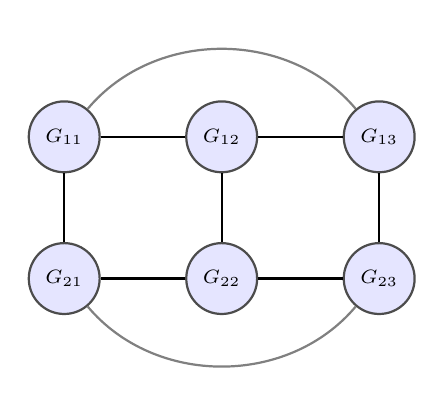
\begin{tikzpicture}[
  g/.style={circle, draw=black!70, thick, minimum size=9mm,
            fill=blue!10, font=\scriptsize}]
  \node[g] (a) at (0,0)   {$G_{11}$};
  \node[g] (b) at (2,0)   {$G_{12}$};
  \node[g] (c) at (4,0)   {$G_{13}$};
  \node[g] (d) at (0,-1.8){$G_{21}$};
  \node[g] (e) at (2,-1.8){$G_{22}$};
  \node[g] (f) at (4,-1.8){$G_{23}$};
  \draw[thick] (a)--(b); \draw[thick] (b)--(c);
  \draw[thick] (d)--(e); \draw[thick] (e)--(f);
  \draw[thick] (a)--(d); \draw[thick] (b)--(e); \draw[thick] (c)--(f);
  \draw[thick, black!50] (a) to[bend left=50] (c);
  \draw[thick, black!50] (d) to[bend right=50] (f);
\end{tikzpicture}
\par\smallskip
{\small A $2\times 3$ torus: the grey wrap-around links close each row
into a ring.}
\end{center}

The resulting topology is that of a \emph{torus} (the boundary
connections close the rings), and Ring-\allreduce\ generalizes naturally:
one performs a ring reduction along the first dimension, then along the
second, and so on. The key architectural consequence is that, despite
growing total bandwidth, \emph{the number of links per node remains
constant}, giving the design its excellent fault-isolation properties.

\subsection{Physical Realization}

\begin{remark}[From logical to physical]
The logical ring is realized physically in different ways at different
scales. Within a single server, GPUs may share a motherboard with direct
peer-to-peer interconnects (NVLink, \href{https://www.graphcore.ai/}{Graphcore}'s
IPU-Links). Across a rack, servers communicate via a Top-of-Rack (ToR)
switch; if the ToR is cheap, the horizontal edges of the logical topology
become the bottleneck of the entire system. Across data centers,
specialized high-speed networking---\textsc{InfiniBand} at
$200$\,Gbps, for instance, via Mellanox (now NVIDIA) network cards---carries
the load. At every level the cost of the \emph{connection} is nontrivial:
a single high-end NIC of an older generation still commands prices in the
range of \$1{,}000--\$1{,}200.
\end{remark}

%%%%%%%%%%%%%%%%%%%%%%%%%%%%%%%%%%%%%%%%%%%%%%%%%%%%%%%%%%%%%%%%%%%%%%%%
\section{Decentralized Alternatives: Parameter Servers and Gossip}
%%%%%%%%%%%%%%%%%%%%%%%%%%%%%%%%%%%%%%%%%%%%%%%%%%%%%%%%%%%%%%%%%%%%%%%%

\allreduce\ is elegant but insists on global synchrony: every device must
arrive at the collective before any may leave. When devices are
heterogeneous, or when the network is flaky, or when stragglers dominate
(each GPU has its own processing time and network delays, so the
synchronous step is as slow as the slowest worker\footnote{The slides
make this point with the same all-reduce schematic, citing
\url{https://arxiv.org/abs/1706.02677}.}), other patterns become
attractive.

\subsection{The Parameter Server}

A \emph{parameter server} (PS) is a dedicated machine that stores the
master copy of $\theta$ and mediates all updates. Workers pull $\theta$,
compute gradients, and push them back; the PS aggregates and updates. The
architecture is described in Li et al.'s
\href{https://www.cs.cmu.edu/~muli/file/parameter_server_osdi14.pdf}{OSDI
2014 paper}.

\begin{center}
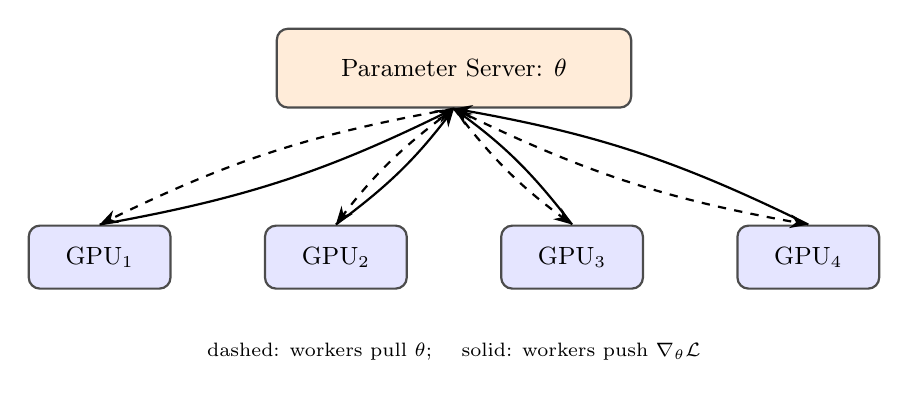
\begin{tikzpicture}[
  ps/.style={rectangle, rounded corners, draw=black!70, thick,
             fill=orange!15, minimum width=4.5cm, minimum height=1cm,
             font=\small},
  w/.style ={rectangle, rounded corners, draw=black!70, thick,
             fill=blue!10, minimum width=1.8cm, minimum height=.8cm,
             font=\small},
  arr/.style={-Stealth, thick}]
  \node[ps] (ps) at (0,2.4) {Parameter Server: $\theta$};
  \node[w] (w1) at (-4.5, 0) {$\GPU{1}$};
  \node[w] (w2) at (-1.5, 0) {$\GPU{2}$};
  \node[w] (w3) at ( 1.5, 0) {$\GPU{3}$};
  \node[w] (w4) at ( 4.5, 0) {$\GPU{4}$};
  \foreach \w in {w1,w2,w3,w4} {
    \draw[arr, dashed] (ps.south) to[bend right=8] (\w.north);
    \draw[arr] (\w.north) to[bend right=8] (ps.south);
  }
  \node[font=\scriptsize, align=left] at (0,-1.2)
    {dashed: workers pull $\theta$; \quad solid: workers push $\grad\Loss$};
\end{tikzpicture}
\end{center}

\begin{description}[leftmargin=1.5em, style=nextline]
  \item[Synchronous mode.] The PS waits for all workers before updating.
        Correct but straggler-bound.
  \item[Asynchronous mode.] Workers push whenever ready, and the PS
        applies updates on arrival. This removes waiting but introduces
        \emph{stale gradients}: a worker's gradient may be computed from a
        version of $\theta$ that is already several updates old by the
        time it is applied. Removing the synchronization step altogether
        is the idea behind
        \href{https://arxiv.org/abs/1106.5730}{\textsc{Hogwild!}}.
\end{description}

\begin{remark}[On stale gradients]
A stale update is, strictly speaking, wrong: it moves $\theta$ in the
direction of a gradient that belongs to a point the trajectory has already
left. But if the step size is small and the optimizer is well-tuned, the
error is bounded, and the throughput gained by eliminating idle time more
than compensates. Convergence may be slowed, but rarely destroyed. This is
a textbook example of the ``controlled relaxation'' philosophy introduced
at the start of these notes.
\end{remark}

Notable implementations include \textsc{BytePS}, as well as sharded
parameter servers whose throughput can rival---and in specific regimes
outstrip---ring-based \allreduce\ systems such as \textsc{Horovod}. The
practical drawback, as the slides stress, is that parameter servers must
ingest enormous volumes of data over the course of training.

\subsection{Gossip Protocols}

A \emph{gossip} protocol dispenses with the central server entirely. Each
worker communicates only with a small neighbourhood, and weights are
reconciled by repeated local averaging. The classical reference for
gossip-style averaging is Boyd et al.\
(\href{https://tinyurl.com/boyd-gossip-2006}{2006}); the lecture also
points to the study ``Can Decentralized Algorithms Outperform Centralized
Algorithms?''\footnote{\url{https://tinyurl.com/can-dsgd-outperform}} for
the claim that gossip-based SGD can beat \allreduce.

\begin{definition}[Gossip averaging step]
Let $x_i^{(k)}$ denote the parameter vector at node $i$ and step $k$, and
let $N_i$ be the set of $i$'s neighbours. A gossip step computes
\[
   x_i^{(k+1)} \;=\; \sum_{j \in \{i\} \cup N_i} w_{ij}^{(k)}\, x_j^{(k)},
   \qquad \sum_j w_{ij}^{(k)} = 1.
\]
Under mild connectivity conditions, iterating this rule drives all $x_i$
toward a common consensus value.
\end{definition}

\begin{center}
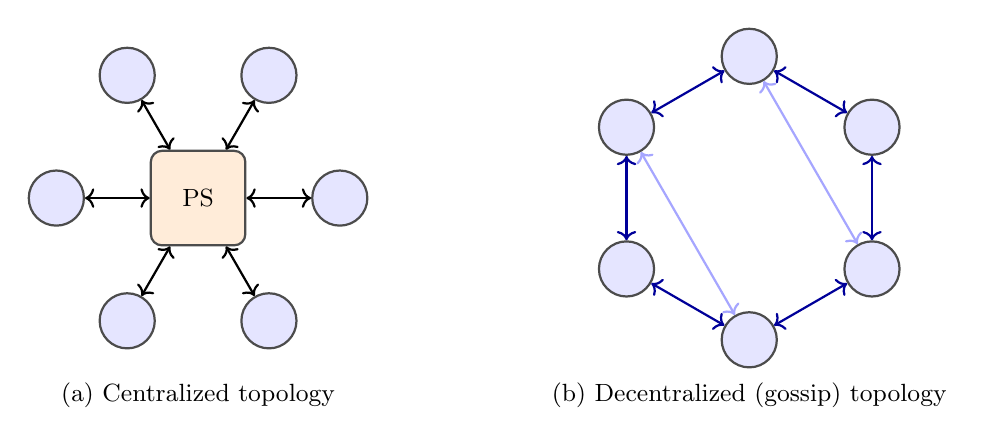
\begin{tikzpicture}[
  n/.style={circle, draw=black!70, thick, minimum size=7mm,
            font=\scriptsize, fill=blue!10}]
  % (a) centralized
  \begin{scope}[xshift=0cm]
    \node[rectangle, rounded corners, draw=black!70, thick, fill=orange!15,
          minimum size=1.2cm, font=\small] (ps) at (0,0) {PS};
    \foreach \a/\name in {0/s1,60/s2,120/s3,180/s4,240/s5,300/s6} {
      \node[n] (\name) at (\a:1.8) {};
      \draw[<->, thick] (\name) -- (ps);
    }
    \node at (0,-2.5) {\small (a) Centralized topology};
  \end{scope}
  % (b) decentralized
  \begin{scope}[xshift=7cm]
    \foreach \a/\name in {90/a,30/b,-30/c,-90/d,-150/e,150/f} {
      \node[n] (\name) at (\a:1.8) {};
    }
    \draw[<->, thick, blue!60!black] (a)--(b); \draw[<->, thick, blue!60!black] (b)--(c);
    \draw[<->, thick, blue!60!black] (c)--(d); \draw[<->, thick, blue!60!black] (d)--(e);
    \draw[<->, thick, blue!60!black] (e)--(f); \draw[<->, thick, blue!60!black] (f)--(a);
    \draw[<->, thick, blue!35] (a)--(c); \draw[<->, thick, blue!35] (d)--(f);
    \node at (0,-2.5) {\small (b) Decentralized (gossip) topology};
  \end{scope}
\end{tikzpicture}
\end{center}

\subsubsection*{Convergence and the Graph}

The analysis of gossip algorithms is, at heart, spectral graph theory.
Three quantities are decisive.

\begin{definition}[Graph degrees, diameter, and mixing time]
For a directed graph $G = (V,E)$ and a node $v$:
\begin{itemize}[leftmargin=1.5em, itemsep=2pt]
  \item the \emph{in-degree} $d_{\text{in}}(v)$ is the number of edges
        entering $v$, and similarly $d_{\text{out}}(v)$ for outgoing
        edges;
  \item the \emph{distance} $d(u,v)$ is the length of the shortest path
        from $u$ to $v$, and the \emph{diameter} is
        $\operatorname{diam}(G) = \max_{u,v} d(u,v)$;
  \item the \emph{mixing time} $\tau_{\text{mix}}$ is the number of steps
        a random walk requires to approach its stationary distribution; it
        encodes how quickly local information becomes global.
\end{itemize}
\end{definition}

Small diameter and small mixing time both favour fast convergence, but
they are not equivalent. A graph may have small diameter yet poor mixing
if its spectral gap is small. For \emph{directed exponential graphs}---in
which the out-degree of each node follows a geometric progression
($1, 2, 4, 8,\ldots$)---average path length turns out to be a better
predictor of convergence speed than diameter alone. Recent results
(Beznosikov, Kovalov, and Gorbunov) analyze convergence rates in
precisely these regimes.

\subsection{Stochastic Gradient Push}

The canonical decentralized algorithm is \textbf{Stochastic Gradient
Push} (\textsc{Sgp}; see
\href{https://arxiv.org/abs/1811.10792}{arXiv:1811.10792}). Each node
maintains two quantities: an unnormalized state $x_i$ and a scalar weight
$w_i$. The node's current estimate of $\theta$ is the ratio
$z_i = x_i / w_i$.

\begin{center}
\fbox{\begin{minipage}{0.92\textwidth}
\textbf{Algorithm 1}\;\;Stochastic Gradient Push (\textsc{Sgp}).

\smallskip
\textbf{Require:} learning rate $\gamma > 0$; initial
$x_i^{(0)} = z_i^{(0)} \in \mathbb{R}^d$; initial weight $w_i^{(0)} = 1$
for all $i \in \{1,\ldots,n\}$.

\smallskip
\textbf{For} $k = 0, 1, \ldots, K-1$, at each node $i$:
\begin{enumerate}[leftmargin=1.8em, itemsep=2pt, label=\arabic*.]
  \item Sample a mini-batch $\xi_i^{(k)} \sim \mathcal{D}_i$ from the
        local distribution.
  \item Compute the local stochastic gradient
        $\nabla F_i\!\left(z_i^{(k)}; \xi_i^{(k)}\right)$.
  \item Local step:
        $\tilde x_i \;=\; x_i^{(k)} - \gamma\, w_i^{(k)}\,
         \nabla F_i\!\left(z_i^{(k)}; \xi_i^{(k)}\right)$.
  \item Send $\left(p_{ij}^{(k)}\tilde x_i,\; p_{ij}^{(k)} w_i^{(k)}\right)$
        to each out-neighbour $j$.
  \item Receive
        $\left(p_{ji}^{(k)}\tilde x_j,\; p_{ji}^{(k)} w_j^{(k)}\right)$
        from each in-neighbour.
  \item Aggregate:
        \[
          x_i^{(k+1)} = \sum_{j \in N_{\text{in}}(i) \cup \{i\}} p_{ji}^{(k)} \tilde x_j,
          \qquad
          w_i^{(k+1)} = \sum_{j \in N_{\text{in}}(i) \cup \{i\}} p_{ji}^{(k)} w_j^{(k)}.
        \]
  \item Normalize: $z_i^{(k+1)} = x_i^{(k+1)} / w_i^{(k+1)}$.
\end{enumerate}
\end{minipage}}
\end{center}

The factor $w_i$ absorbs the asymmetry of a general directed graph: even
if column-stochasticity of the mixing matrix $P^{(k)}$ is not maintained,
dividing by $w_i$ yields an unbiased consensus estimate. The algorithm is
a minor modification of ordinary SGD---one extra scalar per node, one
extra exchange---and in practice converges remarkably close to the
idealized synchronous \allreduce\ baseline, often in strictly less
wall-clock time.

%%%%%%%%%%%%%%%%%%%%%%%%%%%%%%%%%%%%%%%%%%%%%%%%%%%%%%%%%%%%%%%%%%%%%%%%
\section{Communication Compression}
%%%%%%%%%%%%%%%%%%%%%%%%%%%%%%%%%%%%%%%%%%%%%%%%%%%%%%%%%%%%%%%%%%%%%%%%

Every pattern so far has taken for granted that the \emph{content} of
messages is the full-precision gradient. For very large models and
bandwidth-constrained links, this is extravagant. Communication
compression seeks to transmit less without harming convergence.

\subsection{Quantized Communication}

The simplest idea is to cast gradients to low precision before
transmission. A practical scheme is \emph{hybrid precision}: $32$-bit
arithmetic for the weight update and the error buffer, but only $8$-bit
(or even $1$-bit) on the wire. The delicate question is which $8$-bit
\emph{format} to use: linear quantization, mantissa-biased floating point,
a static binary bisection tree, a dynamic tree adaptive to the
distribution of the current gradient, and so on. Each allocates its bits
differently between range and precision; the optimum depends on gradient
statistics. The scheme and the comparison of formats are from
\href{https://arxiv.org/abs/1511.04561}{arXiv:1511.04561}, whose headline
result---as summarized on the slide---is quality matching float16 with
$8$-bit communication and $32$-bit computation.

\begin{center}
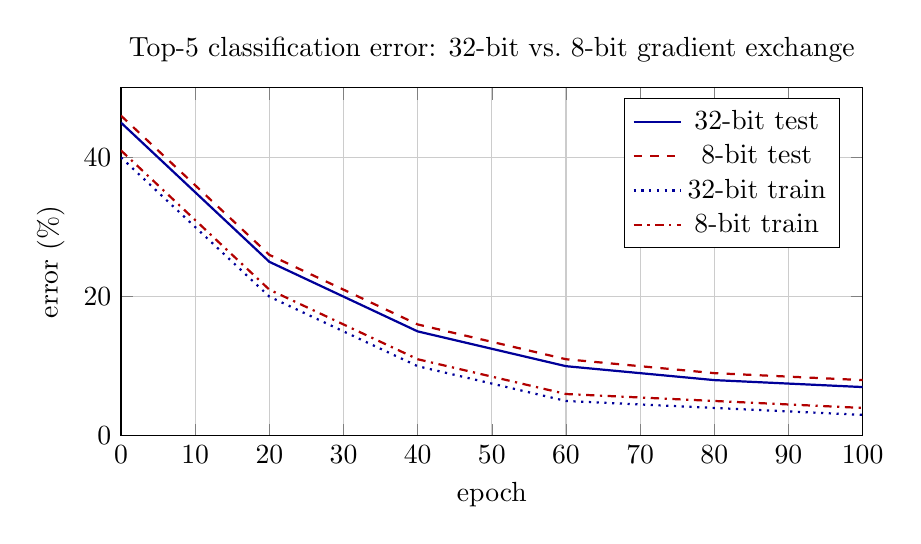
\begin{tikzpicture}
\begin{axis}[
    width=11cm, height=6cm,
    title={Top-5 classification error: 32-bit vs.\ 8-bit gradient exchange},
    xlabel={epoch}, ylabel={error (\%)},
    xmin=0, xmax=100, ymin=0, ymax=50,
    legend pos=north east,
    grid=both,
    major grid style={black!20},
    minor grid style={black!8}]
\addplot[color=blue!60!black, thick] coordinates
    {(0,45)(20,25)(40,15)(60,10)(80,8)(100,7)};
\addplot[color=red!70!black, thick, dashed] coordinates
    {(0,46)(20,26)(40,16)(60,11)(80,9)(100,8)};
\addplot[color=blue!60!black, thick, dotted] coordinates
    {(0,40)(20,20)(40,10)(60,5)(80,4)(100,3)};
\addplot[color=red!70!black, thick, dashdotted] coordinates
    {(0,41)(20,21)(40,11)(60,6)(80,5)(100,4)};
\legend{32-bit test, 8-bit test, 32-bit train, 8-bit train}
\end{axis}
\end{tikzpicture}
\par\smallskip
{\small Schematic illustration; values are illustrative, not taken from the
paper.}
\end{center}

The plot tells a characteristic story: with a reasonable quantization
scheme, $8$-bit communication tracks the full-precision baseline so
closely that the curves are visually indistinguishable.

\subsection{Error Feedback}

Na\"ive aggressive compression---$1$-bit sign quantization, top-$k$
sparsification at, say, $k=5\%$---is not sufficient on its own. Small but
persistent gradient components may never cross the compression threshold
and will be dropped forever, biasing the trajectory. The fix is an
\emph{error-feedback} (EF) loop: whatever the compressor discarded at
step $k$ is remembered and added back at step $k+1$.

\begin{definition}[Compression error]
Let $\mathbf{g}$ be the locally computed gradient and $\mathbf{C}(\cdot)$ a
(possibly stochastic) compression operator. The \emph{compression error}
is
\[
   \mathbf{e} \;=\; \mathbf{g} \;-\; \mathbf{C}(\mathbf{g}).
\]
\end{definition}

\begin{center}
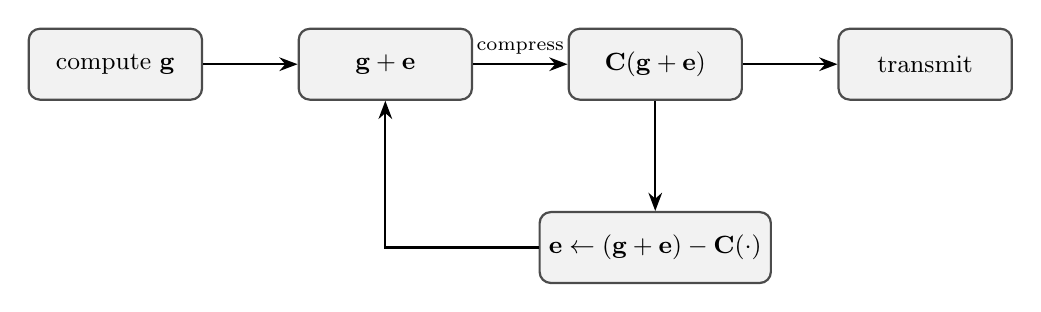
\begin{tikzpicture}[
  b/.style={rectangle, rounded corners, draw=black!70, thick, fill=gray!10,
            minimum width=2.2cm, minimum height=.9cm, font=\small},
  arr/.style={-Stealth, thick},
  node distance=14mm and 12mm]
  \node[b] (grad) {compute $\mathbf{g}$};
  \node[b, right=of grad] (add)  {$\mathbf{g} + \mathbf{e}$};
  \node[b, right=of add]  (comp) {$\mathbf{C}(\mathbf{g}+\mathbf{e})$};
  \node[b, right=of comp] (send) {transmit};
  \node[b, below=of comp] (err)  {$\mathbf{e} \leftarrow (\mathbf{g}+\mathbf{e}) - \mathbf{C}(\cdot)$};
  \draw[arr] (grad) -- (add);
  \draw[arr] (add)  -- node[above, font=\scriptsize]{compress} (comp);
  \draw[arr] (comp) -- (send);
  \draw[arr] (comp) -- (err);
  \draw[arr] (err.west) -| (add.south);
\end{tikzpicture}
\end{center}

Because the residual $\mathbf{e}$ accumulates, small components eventually
grow large enough to survive the compressor, and the model's updates
converge to what they would have been under full precision---only over a
slightly longer number of steps.

\begin{remark}[Memory trade-off]
Error feedback is essentially free in \emph{communication}, but it is not
free in \emph{memory}: the buffer $\mathbf{e}$ has the same dimension as
the gradient and, to avoid compounding roundoff, is typically stored in
full precision. Radical bandwidth reductions (for example, $1$-bit
\textsc{Adam}) thus trade network for local RAM.
\end{remark}

\subsection{PowerSGD}

\textsc{PowerSGD} pushes the idea further by exploiting the observation
that deep-learning gradient matrices are approximately low-rank. At each
step it computes a rank-$r$ factorization $\mathbf{g} \approx P Q^{\top}$
(via a cheap power iteration) and transmits only the two thin matrices
$P$ and $Q$. Combined with error feedback, the resulting gradient
estimator is unbiased in the limit and supports extremely aggressive
compression ratios. In PyTorch, the integration is idiomatic: one
registers a communication \emph{hook} on the
\texttt{DistributedDataParallel} wrapper that intercepts gradients before
the \allreduce, applies compression, and restores the residual after.

\begin{remark}[Classical references]
The foundational papers are
\href{https://arxiv.org/abs/1901.09847}{Karimireddy et al., ``Error
Feedback Fixes SignSGD and Other Gradient Compression Schemes''
(arXiv:1901.09847)}, and
\href{https://arxiv.org/abs/1905.13727}{Vogels, Karimireddy, Jaggi,
``PowerSGD: Practical Low-Rank Gradient Compression for Distributed
Optimization'' (arXiv:1905.13727)}. The slides also point to
\href{https://arxiv.org/abs/2106.05203}{arXiv:2106.05203} (``better
EF'21'') and \href{https://arxiv.org/abs/2110.03294}{arXiv:2110.03294}
(``more EF'21'') for further reading on error feedback.
\end{remark}

%%%%%%%%%%%%%%%%%%%%%%%%%%%%%%%%%%%%%%%%%%%%%%%%%%%%%%%%%%%%%%%%%%%%%%%%
\section{Implementation in PyTorch}
%%%%%%%%%%%%%%%%%%%%%%%%%%%%%%%%%%%%%%%%%%%%%%%%%%%%%%%%%%%%%%%%%%%%%%%%

\subsection{\texttt{DistributedDataParallel}}

In PyTorch, the idiomatic realization of everything above is the
\texttt{DistributedDataParallel} (DDP) wrapper, launched via
\verb|torchrun --nproc_per_node=N train.py|. A typical
\texttt{setup\_ddp} routine performs four duties:

\begin{enumerate}[leftmargin=1.8em, itemsep=2pt]
  \item \textbf{Process group initialization.} A logical group of the $N$
        processes is created so that collective operations know their
        membership.
  \item \textbf{Distributed sampler.} A \texttt{DistributedSampler}
        partitions the dataset so that each process sees a distinct,
        non-overlapping shard---the scattering of the batch $X$ of
        Section~3 made concrete.
  \item \textbf{Model wrapping.} The model, after being moved to its
        assigned GPU, is wrapped in \texttt{DistributedDataParallel},
        which manages parameter registration, buffer synchronization, and
        gradient hooks.
  \item \textbf{Synchronization backend.} The chosen backend
        (\textsc{Nccl} for GPU clusters, \textsc{Gloo} for CPU) performs
        ring-\allreduce\ on gradients during the backward pass.
\end{enumerate}

Manual synchronization is possible but rarely advisable; DDP handles not
only the reduction but the subtle bookkeeping of bucket fusion, overlap
with the backward pass, and uneven-input handling. See
the
\href{https://tinyurl.com/distributed-dp}{introduction to PyTorch
distributed} as a starting point (it can also be worked through in about
fifteen minutes).

\subsection{Scale-Dependent Recommendations}

Different regimes call for different tools:

\begin{itemize}[leftmargin=1.5em, itemsep=2pt]
  \item \textbf{2--4 GPUs on a single host.} The na\"ive
        \href{https://tinyurl.com/torch-data-parallel}{\texttt{nn.DataParallel}}
        module suffices when simplicity matters more than peak
        throughput.
  \item \textbf{4+ GPUs, single or multi-host.} DDP or
        \href{https://github.com/horovod/horovod}{\textsc{Horovod}} are
        the appropriate choices, backed by high-speed interconnects
        (\textsc{InfiniBand} between hosts, \textsc{Nvlink} within).
  \item \textbf{Very large clusters.} Elastic frameworks such as
        \href{https://tinyurl.com/torch-elastic}{\texttt{torch-elastic}}
        allow nodes to join and leave without restarting training; the
        \href{https://arxiv.org/abs/1904.00962}{\textsc{Lamb}} optimizer
        stabilizes learning at batch sizes in the millions.
\end{itemize}

\subsection{Orthogonal Concerns}

Several issues live alongside, rather than inside, the data-parallel
abstraction proper:

\begin{description}[leftmargin=1.5em, style=nextline]
  \item[Memory constraints.] Each worker holds a full replica of $\theta$.
    Models that do not fit on a single GPU demand \emph{model
    parallelism} or sharded-weight schemes (ZeRO, FSDP).
  \item[Large-batch generalization.] Data parallelism tends to push the
    effective batch size upward; beyond a critical size, generalization
    deteriorates. Specialized optimizers (\textsc{Lamb}, \textsc{Lars})
    and careful warm-up schedules are the standard remedy.
  \item[Heterogeneous networks.] When links have wildly different
    bandwidths---a common situation across data centers---graph-aware
    scheduling and asynchronous methods become preferable.
  \item[Non-IID data.] When per-worker data distributions differ, the mean
    of local gradients is no longer an unbiased estimate of the global
    gradient, and extra care (or federated-learning techniques) is
    required.
  \item[Fault tolerance.] Over thousands of GPUs, failures are a
    certainty, not a possibility; both synchronous (with straggler
    dropping) and asynchronous modes admit fault-tolerant realizations.
\end{description}

\subsection{Group \allreduce: The Best of Both Worlds}

A hybrid pattern combines gossip's flexibility with \allreduce's
precision. A gossip protocol is used not to converge weights, but to
\emph{form small groups} of workers; within each group, a short
\allreduce\ is executed. The pattern is robust to failures---the collapse
of one group does not affect the others---and scales gracefully in
heterogeneous networks. It may be viewed as a randomized cousin of
torus-\allreduce. The core idea, as stated on the slides, is to run
all-reduce in independent groups, so that one synchronizes only with a
small group of workers, and to swap groupmates between iterations; the
experiments (up to $1024$ GPUs, with natural or emulated network latency)
are reported in
\href{https://arxiv.org/abs/2005.00124}{arXiv:2005.00124}.

\begin{center}
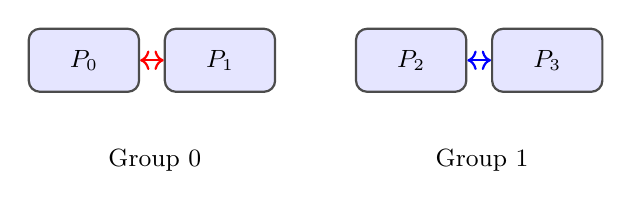
\begin{tikzpicture}[
  p/.style={rectangle, rounded corners, draw=black!70, thick,
            minimum width=1.4cm, minimum height=.8cm,
            fill=blue!10, font=\small}]
  \node[p] (P0) {$P_0$}; \node[p, right=3mm of P0] (P1) {$P_1$};
  \node[p, right=10mm of P1] (P2) {$P_2$}; \node[p, right=3mm of P2] (P3) {$P_3$};
  \draw[<->, thick, red]  (P0) -- (P1);
  \draw[<->, thick, blue] (P2) -- (P3);
  \node[below=6mm of P0, xshift=9mm] {\small Group 0};
  \node[below=6mm of P2, xshift=9mm] {\small Group 1};
\end{tikzpicture}
\end{center}

A useful principle emerges. \emph{The shape of the algorithm must follow
the shape of the hardware.} A tree is right when latency is the enemy; a
ring is right when bandwidth is; a torus is right when both are; a gossip
mesh is right when neither the hardware nor the trust relationships are
uniform. When designing a distributed-training system, identify the
binding constraint first, and pick the pattern that dissolves it.

\medskip
\noindent\textbf{Further reading.} PyTorch's
\texttt{DistributedDataParallel} documentation; the
\href{https://github.com/horovod/horovod}{\textsc{Horovod}} project page;
the \textsc{PowerSGD} and error-feedback papers cited above; and---for
those interested in large-batch optimization---the
\href{https://arxiv.org/abs/1904.00962}{\textsc{Lamb} paper
(arXiv:1904.00962)}.

\end{document}